\begin{frame}{Motivation}
	\begin{itemize}
		\item Speed up the tedious process of hyperparameter optimisation
		\item Overcome the issue of optimal architecture being highly problem dependent
		\item Avoid biased decision of an expert user
		\item Utilize the baf job submission structure to efficiently run large samples of small optimisation jobs
	\end{itemize}
\end{frame}

\begin{frame}{Theory}
	\begin{itemize}
		\item Code inspired by \cite{naranjo}
		\item Use a $(\lambda + \mu)$ scheme.
		\item $\lambda$ individuals per generation
		\item $\mu$ individuals selected to create the next generation
	\end{itemize}
	\begin{figure}
    	\centering
		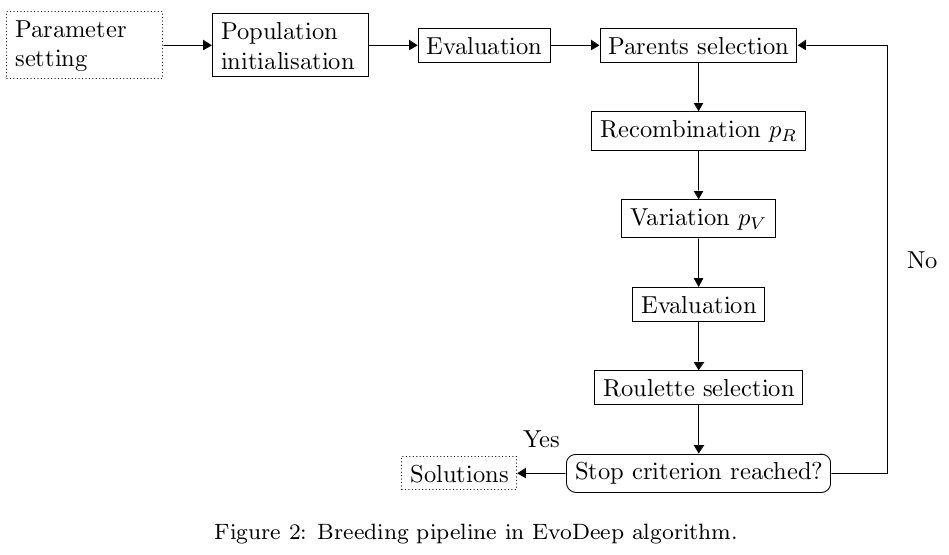
\includegraphics[width=0.8\textwidth]{breed.png}
    \end{figure}
\end{frame}

\begin{frame}{Baf setup}
	\begin{enumerate}
		\item A bash script submits a badge of jobs from the local machine
		\item The script waits for all jobs to finish
		\item The jobs are evaluated based on AUC and Accuracy
		\item Based on the evaluation, a new set of jobs is created
		\item Remnants of the old submission are removed to avoid exceeding quota
	\end{enumerate}
\end{frame}

\begin{frame}{Early results}
	\begin{itemize}
		\item Testing tZ versus ttbar
		\item Tested for Lorentz-Invariant and basic kinematic variables
		\item Testing on nodes, layers, learning rate, dropout
		\item The network ends around:
		\item Testing for similarity of final paramters. Even for small test samples the parameters are very similar
		\item Plots soon to come, unfortunately I had some plotting issues that are now fixed
	\end{itemize}
\end{frame}

\begin{frame}{Conclusion and future steps}
	\begin{itemize}
		\item Running smoothly on baf for all test runs
		\item The network is approaching a reasonable order of magnitude and getting closer every single step
		\item Unreasonable genotypes are discarded
		\item Biggest impact made by epochs and metrics
		\item Weight ini has to be checked
		\item Starting parameters have to bet set. Lately some runs resulted in bad parameters
	\end{itemize}
\end{frame}

